\newpage
\chapter{AI-BLOCKCHAIN HYBRID PHISHING DEFENSE}

\section{DESCRIPTION}

\hspace{1cm}\textbf{Hybrid Phishing Defense} is an intelligent, AI-powered cybersecurity assistant designed to monitor, analyze, and prevent malicious web browsing in real time. It leverages natural language processing and deep learning techniques to detect zero-day phishing attempts, helping individuals and organizations browse safely without relying on outdated, centralized blacklists. 

The system uses advanced deep learning architectures such as \textit{CNN} and \textit{LSTM} to extract lexical features, identify structural URL anomalies, and analyze host-based patterns across web sessions. Through these insights, the system provides users with immediate feedback on domain safety, ensuring that every web request is authenticated against malicious indicators. 

The platform integrates an \textbf{Adaptive Threat Detection Core} that learns from global phishing data and adjusts risk scoring algorithms dynamically. By combining real-time visual alerts, AI-based threat prediction, and immutable blockchain logging, the system creates a personalized, secure, and decentralized browsing environment. 

Additionally, the system offers detailed weekly security reports, personalized safe-browsing suggestions, and dynamic threat modifications to help users protect their digital assets efficiently. The intuitive browser dashboard allows users to view their protected sessions, while security analysts or administrators can monitor global threat insights for multiple network nodes. The system transforms traditional reactive security into a smart, AI-driven, and decentralized protection solution. It also emphasizes user accessibility by offering multi-platform browser compatibility, allowing seamless operation across desktop and mobile environments. Furthermore, its privacy-focused design ensures that all browsing data is processed securely on-device, maintaining user confidentiality while delivering precise, real-time threat insights.

\vspace{0.5cm}

\section{ARCHITECTURE}

\hspace{1cm}The architecture of the Hybrid Phishing Defense system is structured around the modular integration of user browser interaction, AI-driven threat analysis, and decentralized ledger technology. The system starts with the browser extension input that captures real-time URL navigation, followed by feature extraction, lexical analysis, and risk assessment modules. These modules interact with the adaptive threat detection core, which personalizes security feedback and calculates a probability score. The processed threat data is stored immutably on the blockchain for global analytics, generating comprehensive security reports for both end-users and network administrators.

\vspace{0.4cm}
\begin{figure}[htbp]
  \centering
  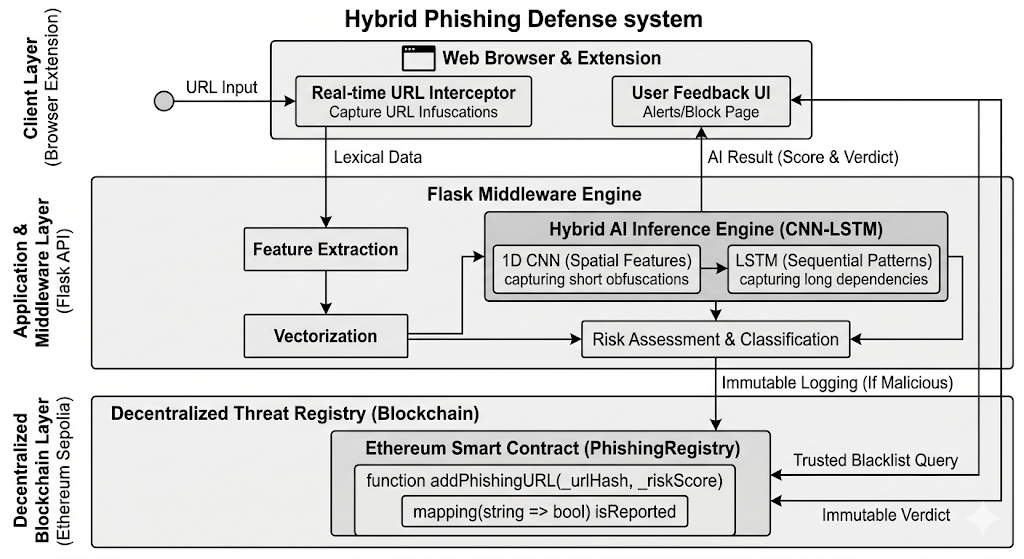
\includegraphics[width=1\textwidth]{assets/Architecture.png}
  \captionsetup{justification=centering}
  \caption{Architecture of the proposed Hybrid Phishing Defense system.}
  \label{fig:architecture}
\end{figure}
The architecture ensures seamless coordination between real-time URL interception and decentralized intelligent analytics. Each component is designed to operate both independently and synergistically, allowing flexible scaling and system upgrades. The \textbf{Browser Interception} module continuously streams navigated URLs to the \textbf{Feature Extraction} and \textbf{AI Inference} units, where domain structure and string anomalies are evaluated using CNN-LSTM algorithms. The \textbf{Risk Assessment} module quantifies metrics like phishing probability and zero-day likelihood, forwarding the analyzed data to the \textbf{Adaptive Threat Detection Core}, which dynamically adjusts security parameters. This processed information is permanently stored in the \textbf{Decentralized Threat Registry (Blockchain)}, ensuring a traceable, tamper-proof history of attacks and supporting global trend-based insights. Finally, the \textbf{User Interface} integrates feedback mechanisms such as visual warning overlays, proactive page blocking, and risk dashboards, providing users with actionable security insights in real time.


\section{MODULE DESCRIPTION}

\subsection{ADMIN MODULE}

\hspace{1cm}\textbf{Description:}  
The Admin Module acts as the central management interface for cybersecurity analysts and system administrators, offering a comprehensive suite of tools to oversee and optimize the threat defense network. It facilitates secure Web3 login and access control, allowing authorized personnel to manage smart contract deployments, review flagged domains, and monitor global threat trends. Through integrated analytics, administrators can evaluate AI prediction accuracy, track false positive rates, and assess the effectiveness of the CNN-LSTM detection mechanisms.  

This module also enables the configuration and fine-tuning of feature extraction parameters, neural network weights, and risk score thresholds to ensure accurate and safe browsing experiences. Administrators can upload new training datasets, update heuristic rules, and maintain the decentralized knowledge base that supports real-time feedback. The system provides detailed reports on global phishing campaigns, network usage, and smart contract gas optimization, helping analysts make informed decisions.  

\noindent Additionally, the Admin Module interfaces with the Decentralized Threat Registry to maintain immutable historical records, ensure data integrity, and support long-term cybersecurity tracking. Notifications and consensus tools allow analysts to vote on domain validity, offering expert review on edge-case URLs. Overall, the module ensures operational stability, ledger transparency, and continuous AI model refinement.

\vspace{.8cm}

\textbf{Purpose:}  
To empower cybersecurity analysts and administrators with intelligent tools for managing global threat data, configuring AI behavior, maintaining blockchain integrity, and ensuring the smooth operation of the decentralized security platform across all nodes.  
The module facilitates informed decision-making by providing actionable insights derived from real-time analytics and historical attack trends.  
It supports continuous system refinement through adaptive machine learning feedback loops and smart contract upgradeability.  
By centralizing threat oversight while maintaining decentralized data storage, the Admin Module enhances scalability, accountability, and network resilience across the platform.
\newpage
\begin{figure}[htbp]
  \centering
  \includegraphics[width=1\textwidth]{assets/Admin.png}
  \captionsetup{justification=centering}
  \caption{Admin module interface and workflow of the Hybrid Phishing Defense system.}
  \label{fig:adminmodule}
\end{figure}
 

This flowchart illustrates the architecture of the Admin Management System within the AI cybersecurity platform. It begins with secure Web3 wallet authentication, followed by access to four core modules: \textit{Threat Management}, \textit{Model Configuration}, \textit{Blockchain Analytics \& Reports}, and \textit{System Configuration}. Each module interacts with the \textit{Adaptive Threat Detection Core}, which processes model updates, global reports, and smart contract settings. Verified threat data and processed insights are stored in the centralized \textit{Decentralized Ledger \& Analytics} unit. The diagram highlights a streamlined workflow where administrators oversee network safety, update neural network models, and maintain blockchain integrity through intelligent feedback loops and structured data flow across all components.

\vspace{0.5cm}

\textbf{Key Features:}
\begin{itemize}
    \item Secure Web3 login with cryptographic wallet authentication and role-based access control.
    \item Centralized threat management including domain reviewing, manual flagging, and false-positive resolution.
    \item Real-time analytics and reporting on AI prediction accuracy and zero-day threat detection.
    \item Configuration of CNN-LSTM hyperparameters and adaptive risk thresholds.
    \item Integration with the Adaptive Threat Detection Core for dynamic model retraining and deployment.
\end{itemize}
\subsection{USER MODULE}

\hspace{1cm}\textbf{Description:}  
The User Module is designed to offer a comprehensive, intuitive, and unobtrusive security experience for everyday web users. It begins with the installation of the browser extension and optional Web3 wallet connection, allowing users to define their security strictness, view historical browsing safety, and manage trusted domains. Once initialized, the module uses background scripts to monitor URL navigation and web requests in real time, powered by advanced AI-based feature extraction.  

As users browse the internet, the system continuously analyzes URL structures and domain metadata, identifying obfuscated links and providing immediate corrective feedback through visual overlays, red warning screens, and proactive page blocking. This ensures credential safety, reduces the risk of identity theft, and improves overall digital hygiene. The interface also includes educational prompts regarding why a site was blocked to encourage better security awareness.  

A dynamic dashboard visualizes protection metrics such as total links scanned, threats blocked, risk distributions, and security trends over time. The Adaptive Threat Detection Core personalizes the browsing experience by adjusting scanning intensity and alerting mechanisms based on the user's interaction history and the global blockchain ledger. Users also receive AI-generated safe-browsing suggestions aligned with current emerging threats. The module is designed to be lightweight and highly responsive, making it suitable for seamless daily browsing without degrading browser performance.

\textbf{Purpose:}  
To empower web users with intelligent tools that guide safe browsing execution, deliver real-time proactive threat blocking, and foster long-term digital security. The module enhances user autonomy, safety, and awareness by combining AI-driven zero-day detection with decentralized transparency and interactive visual warnings.

\vspace{0.5cm}
% Force figure to stay here
\begin{figure}[H]
  \centering
  \includegraphics[width=1\textwidth]{assets/User.png}
  \captionsetup{justification=centering}
  \caption{User module interface and functionality of the Hybrid Phishing Defense system.}
  \label{fig:user}
\end{figure}
\vspace{0.5cm}

The Adaptive Threat Detection System is the central processing unit of the user-facing platform, responsible for analyzing web traffic and delivering instant security verdicts. It integrates data from browser events, URL parsers, and external APIs to perform lexical feature extraction and structural analysis. Based on this, it conducts a risk assessment via the CNN-LSTM engine and interacts with the Ethereum Smart Contracts to verify findings and generate real-time alerts. Historical threat data and zero-day discoveries are pushed to the blockchain to refine future global protections. The system ensures continuous network immunity through dynamic feedback loops and decentralized consensus tracking.

\textbf{Key Features:}  
\begin{itemize}
    \item Real-time URL interception and lexical analysis using background browser scripts.
    \item Adaptive proactive blocking based on AI risk scores and smart contract ledgers.
    \item Integration of historical blockchain data for rapid verification of known threats.
    \item Visual overlay and audio alerts for immediate phishing prevention and user education.
    \item Protection dashboards and security reports for tracking personal browsing safety.
    \item Secure Web3 wallet integration for executing threat-logging transactions.
\end{itemize}